\documentclass[../../Aurora C# unofficial manual.tex]{subfiles}

\begin{document}
	\section{Deleting stars and system bodies}\label{4_deleting_stars_and_bodies}
	Original post can be found
	\href{http://aurora2.pentarch.org/index.php?topic=8495.msg118745#msg118745}{here}.
	\\\\
	
	Deletion of stars or system bodies is straightforward. Click on the target object and then click Delete Body or Delete Star. You will be given two popup warnings and then the object will be deleted. Deleting a star will remove any system bodies in orbit. Deleting a planet will remove any moons of that planet. Any populations on affected system bodies will be deleted. Deleting the primary star is not possible.
	
	When a star is deleted, any remaining stars will be renamed accordingly. For example, if you delete the B component of a primary, the original C component will now become the B component. When a planet or moon is deleted, the orbit numbers of the planets or moons will be adjusted accordingly.
	
	For example, here are the before and after views of the Alpha Centauri-A system when the fourth planet is deleted.
	\begin{figure}[H]
		\centering
		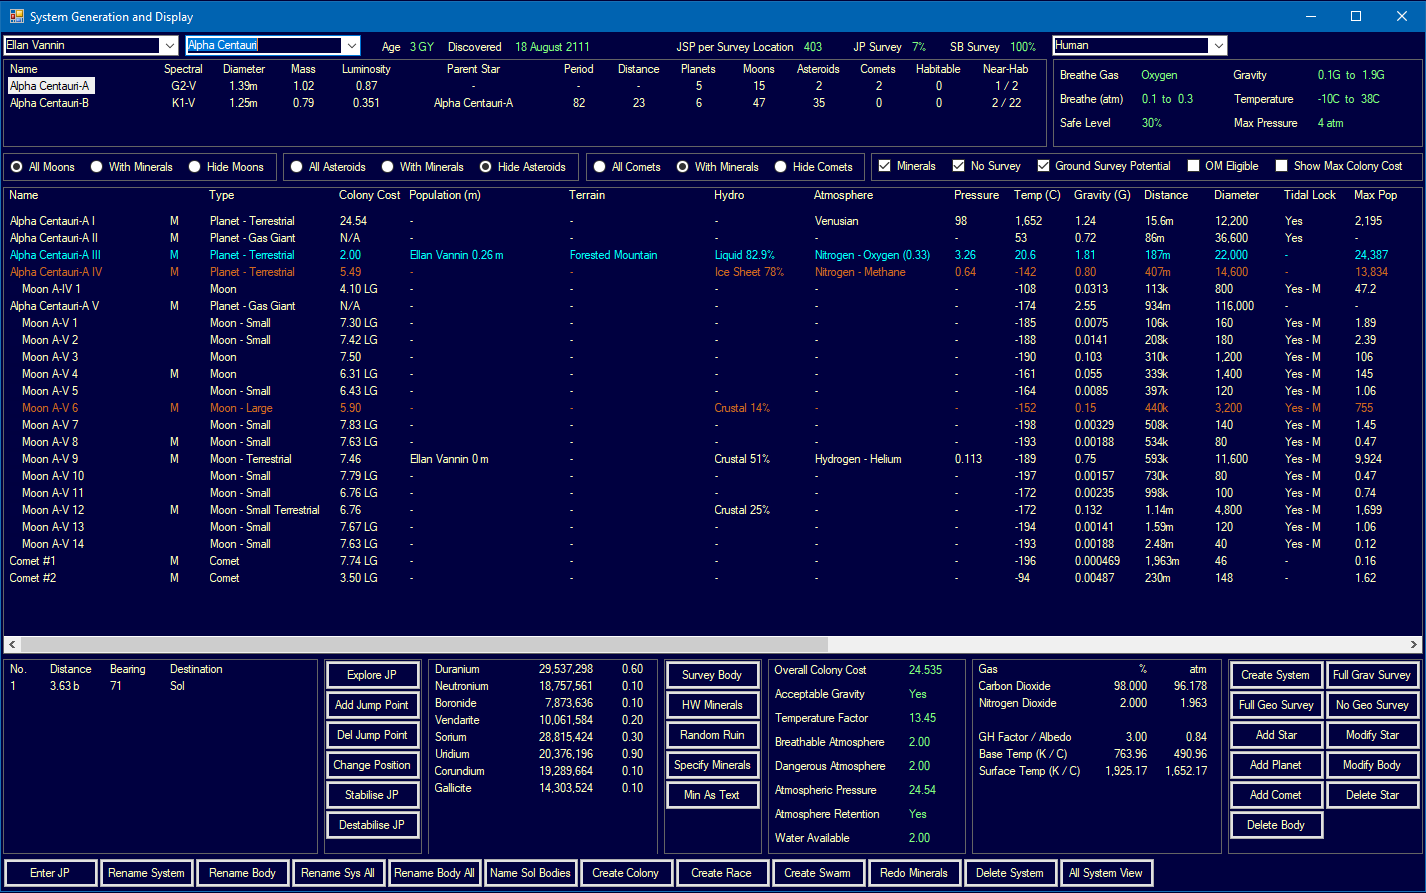
\includegraphics[width=0.95\linewidth]{images/DeletingStarsAndBodies}
		\caption[Deleting Stars And System Bodies]{Deleting Stars And System Bodies}
		\label{fig:deletingstarsandbodies}
	\end{figure}
	\begin{figure}[H]
		\centering
		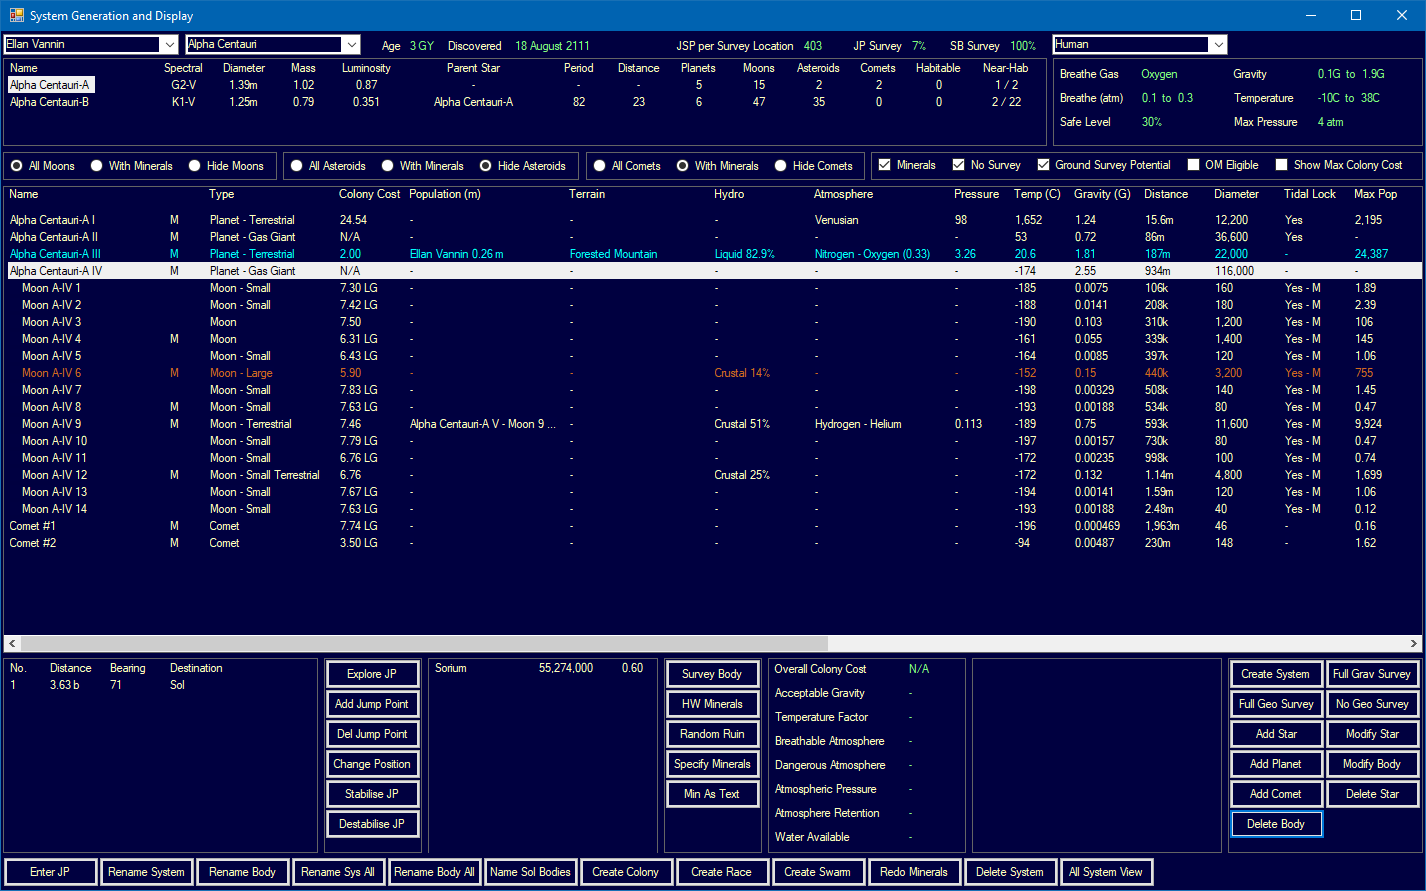
\includegraphics[width=0.95\linewidth]{images/DeletingStarsAndBodies2}
		\caption[Deleting Stars And System Bodies]{Deleting Stars And System Bodies 2}
		\label{fig:deletingstarsandbodies2}
	\end{figure}
\end{document}